%!TeX root=../tese.tex

\chapter{Literatura formal}
\label{cap:literatura-formal}

\section{\citetitle{elsevier} \parencite*{elsevier}}

Esta fonte é uma pesquisa científica revisada por pares e publicada em revistas renomadas, como a \emph{Elsevier}. O objetivo desta pesquisa foi compreender melhor como os desenvolvedores estão utilizando assistentes de IA, porque eles não os usam em determinadas partes de seu fluxo de desenvolvimento e quais aspectos precisam ser aprimorados no futuro.

Para isso, a pesquisa foi realizada com uma quantidade expressiva de pessoas, a coleta de dados incluiu entrevistas com 481 programadores de 71 países diferentes. A amostra da pesquisa é composta principalmente por programadores experientes, dos quais 48,9\% possuem mais de 10 anos de experiência e 28,9\% possuem mais de 15 anos. Do total de participantes, 74,4\% estão empregados em tempo integral em empresas e organizações, enquanto outros atuam parcialmente, são autônomos ou \emph{freelancers}. A maioria (86,7\%) se identifica como desenvolvedor de \emph{software}, mas a amostra também inclui outras posições técnicas relevantes, como engenheiros \emph{DevOps}, arquitetos de \emph{software} e líderes de equipe.

Em particular, foram estudadas as seguintes cinco grandes atividades de engenharia de \emph{software}: implementação de novas funcionalidades, escrita de testes, triagem de erros, refatoração e produção de artefatos em linguagem natural, assim como suas etapas individuais. A pesquisa incluiu 38 perguntas principais, sendo 5 abertas, o que permitiu aos participantes expressarem livremente suas opiniões. A pesquisa obteve 547 respostas completas e, após uma filtragem cuidadosa, foram analisadas 481 respostas.

As principais contribuições dessa pesquisa são:

\begin{itemize}
    \item \textbf{Padrões de uso:} A pesquisa revela que 84,2\% dos participantes utilizam assistentes de IA ocasional ou regularmente, sendo a implementação de novas funcionalidades a atividade mais popular para o uso desses assistentes. Entre as etapas individuais, gerar e resumir código são as mais amplamente utilizadas;
    \item \textbf{Áreas de foco:} Considerando quais atividades os desenvolvedores consideram menos agradáveis e desejam delegar, bem como em quais etapas os assistentes de IA são utilizados, o artigo destaca as áreas nas quais a comunidade acadêmica precisa se concentrar para gerar valor aos usuários. Isso inclui a escrita de testes de forma geral e, em particular, a geração de dados e recursos para testes, assim como a escrita de artefatos em linguagem natural;
    \item \textbf{Razões para não usar IA:} Foram identificados 20 temas distintos que representam diferentes motivos pelos quais os desenvolvedores não utilizam assistentes de IA, com os principais motivos sendo: falta de necessidade de assistência de IA, saída gerada pela IA imprecisa, falta de confiança do usuário e desejo de manter controle, e compreensão insuficiente do contexto pelo assistente de IA. Os dados em detalhes estão na \autoref{tab:razoes_nao_usar};
    \item \textbf{Áreas para melhorias futuras:} Com base na prevalência das diferentes razões, foram formuladas as principais áreas de trabalho futuro necessárias para superar as limitações apontadas pelos respondentes. Entre elas estão a melhoria dos sistemas base, melhor integração no fluxo de trabalho dos desenvolvedores e educação mais ativa dos usuários sobre as capacidades e limitações dos assistentes.
\end{itemize}

\begin{table}[h]
    \centering
    \caption{Temas resultantes nas respostas à pergunta "O que impede você de usar assistentes de IA nas etapas do fluxo de trabalho que você não os utiliza IA?" (\cite{elsevier}).}
    \label{tab:razoes_nao_usar}
    \renewcommand{\arraystretch}{1.2}
    \small
    \rowcolors{2}{gray!15}{white}
    \begin{tabular}{m{12.5cm} c}
        \toprule
        Motivo & Resp. (\%) \\
        \midrule
        Falta de necessidade de assistência de IA & 22.5 \\
        Saída gerada pela IA imprecisa & 17.7 \\
        Falta de confiança do usuário e desejo de ter controle & 15.7 \\
        Falta de compreensão do contexto pelo assistente de IA & 14.4 \\
        Conhecimento limitado do usuário sobre assistentes de IA e suas capacidades & 10.2 \\
        Desejo do usuário de realizar a tarefa sozinho e aprender & 7.3 \\
        Ineficiência de tempo & 5.5 \\
        Saída gerada pela IA não é útil & 4.6 \\
        Políticas da empresa, NDA, etc. & 3.6 \\
        Atitude negativa do usuário em relação à IA & 3.2 \\
        Falta de conformidade com requisitos não funcionais na saída do assistente de IA & 3.2 \\
        Considerações legais e éticas & 3.1 \\
        Desafios de integração e usabilidade da IA em ambientes de desenvolvimento & 3.0 \\
        Falta de acesso & 2.6 \\
        Preocupações com segurança & 2.3 \\
        Limitações na criatividade da IA & 2.2 \\
        Interrupção do fluxo de trabalho & 2.1 \\
        Limitações de conhecimento do modelo de IA & 1.9 \\
        Ineficiência para tarefas específicas & 1.7 \\
        Desafios na comunicação das intenções do usuário ao assistente de IA & 1.0 \\
        \bottomrule
    \end{tabular}
\end{table}

\begin{figure}[h!]
    \caption{Ferramentas utilizadas pelos desenvolvedores (\cite{elsevier}; n = 481)}
    \label{fig:ferramentas_elsevier}
    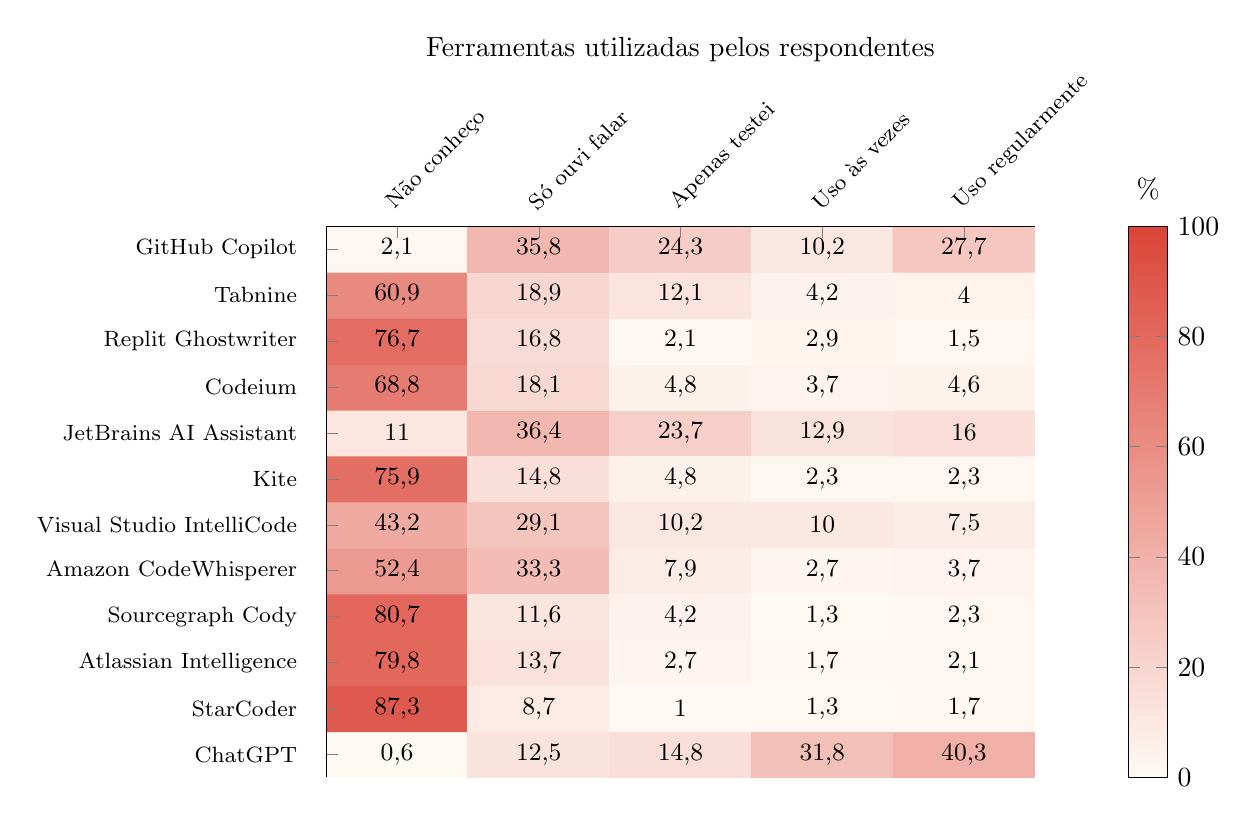
\begin{tikzpicture}
        \begin{axis}[
                /pgf/number format/use comma,
                enlargelimits=false,
                axis on top,
                scale only axis,
                title={Ferramentas utilizadas pelos respondentes},
                title style={
                        yshift=50pt
                    },
                width=9cm,
                height=7cm,
                xmin=0, xmax=5,
                ymin=0, ymax=12,
                xtick={0.5, 1.5, 2.5, 3.5, 4.5},
                ytick={0.5, 1.5, 2.5, 3.5, 4.5, 5.5, 6.5, 7.5, 8.5, 9.5, 10.5, 11.5},
                yticklabels={
                        ChatGPT,
                        StarCoder,
                        Atlassian Intelligence,
                        Sourcegraph Cody,
                        Amazon CodeWhisperer,
                        Visual Studio IntelliCode,
                        Kite,
                        JetBrains AI Assistant,
                        Codeium,
                        Replit Ghostwriter,
                        Tabnine,
                        GitHub Copilot,
                    },
                xticklabels={
                        Não conheço,
                        Só ouvi falar,
                        Apenas testei,
                        Uso às vezes,
                        Uso regularmente
                    },
                xticklabel style={
                        rotate=45,
                        anchor=west,
                        font=\footnotesize,
                        yshift=7pt
                    },
                yticklabel style={
                        font=\footnotesize,
                        align=right,
                        xshift=-7pt
                    },
                axis x line*=top,
                axis y line*=left,
                colorbar,
                colorbar style={
                        title={\%},
                        ytick={0,20,40,60,80,100},
                    },
                colormap={redscale}{
                        rgb255(0cm)=(255, 250, 245);
                        rgb255(1cm)=(219, 68, 55)
                    },
                point meta min=0,
                point meta max=100,
                nodes near coords={
                        \pgfmathprintnumber[fixed, precision=1]{\pgfplotspointmeta}
                    },
                nodes near coords style={
                        font=\bfseries\small,
                        color=black,
                        anchor=center
                    }
            ]
            \addplot [
                matrix plot*,
                mesh/rows=12,
                mesh/cols=5,
                point meta=explicit
            ] coordinates {
                    % ChatGPT
                    (0.5,0.5) [0.6]  (1.5,0.5) [12.5] (2.5,0.5) [14.8] (3.5,0.5) [31.8] (4.5,0.5) [40.3]
                    % StarCoder
                    (0.5,1.5) [87.3] (1.5,1.5) [8.7]  (2.5,1.5) [1.0]  (3.5,1.5) [1.3]  (4.5,1.5) [1.7]
                    % Atlassian Intelligence
                    (0.5,2.5) [79.8] (1.5,2.5) [13.7] (2.5,2.5) [2.7]  (3.5,2.5) [1.7]  (4.5,2.5) [2.1]
                    % Sourcegraph Cody
                    (0.5,3.5) [80.7] (1.5,3.5) [11.6] (2.5,3.5) [4.2]  (3.5,3.5) [1.3]  (4.5,3.5) [2.3]
                    % Amazon CodeWhisperer
                    (0.5,4.5) [52.4] (1.5,4.5) [33.3] (2.5,4.5) [7.9]  (3.5,4.5) [2.7]  (4.5,4.5) [3.7]
                    % Visual Studio IntelliCode
                    (0.5,5.5) [43.2] (1.5,5.5) [29.1] (2.5,5.5) [10.2] (3.5,5.5) [10.0] (4.5,5.5) [7.5]
                    % Kite
                    (0.5,6.5) [75.9] (1.5,6.5) [14.8] (2.5,6.5) [4.8]  (3.5,6.5) [2.3]  (4.5,6.5) [2.3]
                    % JetBrains AI Assistant
                    (0.5,7.5) [11.0] (1.5,7.5) [36.4] (2.5,7.5) [23.7] (3.5,7.5) [12.9] (4.5,7.5) [16.0]
                    % Codeium
                    (0.5,8.5) [68.8] (1.5,8.5) [18.1] (2.5,8.5) [4.8]  (3.5,8.5) [3.7]  (4.5,8.5) [4.6]
                    % Replit Ghostwriter
                    (0.5,9.5) [76.7] (1.5,9.5) [16.8] (2.5,9.5) [2.1]  (3.5,9.5) [2.9]  (4.5,9.5) [1.5]
                    % Tabnine
                    (0.5,10.5) [60.9] (1.5,10.5) [18.9] (2.5,10.5) [12.1] (3.5,10.5) [4.2]  (4.5,10.5) [4.0]
                    % GitHub Copilot
                    (0.5,11.5) [2.1]  (1.5,11.5) [35.8] (2.5,11.5) [24.3] (3.5,11.5) [10.2] (4.5,11.5) [27.7]
                };
        \end{axis}
    \end{tikzpicture}
\end{figure}

O gráfico da \autoref{fig:ferramentas_elsevier} mostra as ferramentas que os respondentes utilizam em seu trabalho. De modo geral, 84,2\% dos participantes mencionaram utilizar ao menos uma ferramenta. Entre as ferramentas mais citadas, destacam-se \emph{ChatGPT} (72,1\%), \emph{GitHub Copilot} (37,9\%), \emph{JetBrains AI Assistant} (28,9\%) e \emph{Visual Studio IntelliCode} (17,5\%). Quanto às demais ferramentas, mais da metade dos respondentes não as conhece. Isso indica que o campo de assistentes de IA é dominado por algumas grandes companhias.

\begin{figure}[h!]
    \includegraphics[width=\textwidth]{delegaria_gosto.png}
    \caption{Gráfico representando quais tarefas do desenvolvimento os desenvolvedores gostam de fazer, quais eles delegariam à IA e qual sua impressão de dificuldade sobre as atividades \parencite{elsevier}.}
    \label{fig:grafico_gosto_delegacao}
\end{figure}

Como mostrado na \autoref{fig:grafico_gosto_delegacao}, implementar novas funcionalidades é a atividade mais agradável para os participantes, com até 86\% dos respondentes avaliando-a positivamente. Também é a atividade menos provável de ser delegada a um assistente de IA, com 48\% dos participantes respondendo negativamente. Por outro lado, escrever testes e produzir artefatos em linguagem natural são as atividades menos agradáveis (46\% de avaliações negativas para testes e 43\% para artefatos), sendo também as que os desenvolvedores mais desejam delegar, 70\% e 66\%, respectivamente.

Refatoração é a segunda atividade mais agradável, com 64\% de avaliações positivas. Mesmo assim, 49\% dos participantes considerariam delegar essa atividade a um assistente de IA. Quanto à triagem de erros, as opiniões são mais divididas: 32\% dos respondentes a consideram desagradável e 36\% agradável, enquanto 34\% não a delegariam e 46\% estariam dispostos a delegá-la a uma IA.

O artigo organiza seus principais resultados em quatro \emph{takeaways}, eles são:

\begin{itemize}
    \item A opinião geral sobre o código fornecido pelos assistentes de IA varia, sendo o aspecto mais positivo a sua usabilidade e o mais negativo a segurança;
    \item Entre as principais atividades estudadas, implementar novas funcionalidades é a mais agradável e a menos propensa a ser delegada a um assistente pelos respondentes, enquanto escrever testes e produzir artefatos em linguagem natural são as mais desagradáveis e as mais propensas a serem delegadas;
    \item As funcionalidades mais utilizadas de assistentes de IA estão associadas a geração e resumo, por exemplo, de códigos, testes, refatorações, artefatos de linguagem natural e correções de erros. Por outro lado, usar a IA para modificar autonomamente o repositório ou utilizá-la para identificar pontos onde novas funcionalidades, testes e refatorações devem ser feitos são usos menos populares, apesar de não serem negligenciáveis entre os respondentes;
    \item Os principais motivos pelos quais os desenvolvedores não usam assistentes de IA são: falta de necessidade, saída gerada pela IA imprecisa, falta de confiança e falta de compreensão do contexto pelo assistente.
\end{itemize}

\section{\citetitle{anssi_2024} \parencite*{anssi_2024}}

O relatório foi elaborado conjuntamente pela \emph{Agence Nationale de la Sécurité des Systèmes d’Information} (ANSSI), agência francesa responsável pela cibersegurança nacional, e pelo \emph{Bundesamt für Sicherheit in der Informationstechnik} (BSI), o Escritório Federal Alemão para Segurança da Informação. Ambas são autoridades governamentais que atuam na definição de diretrizes, recomendações e boas práticas para a proteção de sistemas de informação e infraestrutura digital em seus respectivos países.

A publicação analisa as oportunidades e os riscos associados ao uso de assistentes de programação baseados em IA, tecnologia que já é amplamente adotada em organizações e tende a se tornar parte integrante do desenvolvimento de \emph{software}. O relatório começa com uma introdução conceitual sobre o que são assistentes de código com IA e o objetivo do documento. Em seguida, o texto é dividido em seções temáticas que discutem, separadamente, as oportunidades associadas ao uso dessas ferramentas, os riscos de segurança envolvidos e, por fim, um conjunto de recomendações práticas. A conclusão consolida essas recomendações, segmentando-as por níveis organizacionais (gestão, desenvolvimento e pesquisa), o que confere ao texto um caráter normativo e orientado à aplicação prática, típico de publicações institucionais de órgãos de segurança da informação.

O conteúdo em detalhes do artigo não foi compilado na íntegra neste trabalho, pois é bastante denso e repleto de citações diversas. Em vez disso, seu conteúdo e suas referências serão utilizados diretamente na análise presente no \autoref{cap:analise}.